% -*- coding: utf-8 -*-
\newpage
\section{Current Status of QTAIM in AMS}

To encapsulate the QTAIM code and ensure its accessibility from the various
engines within the suite, we have documented the interconnection of the main
\modules. This modular design not only facilitates integration into existing
workflows but also simplifies future development. Figure~\ref{ams_workflow}
illustrates how \gls{QTAIM} can be invoked within a typical \ams workflow, from
user input through to the final output.

\begin{figure}[h]
  \centering
  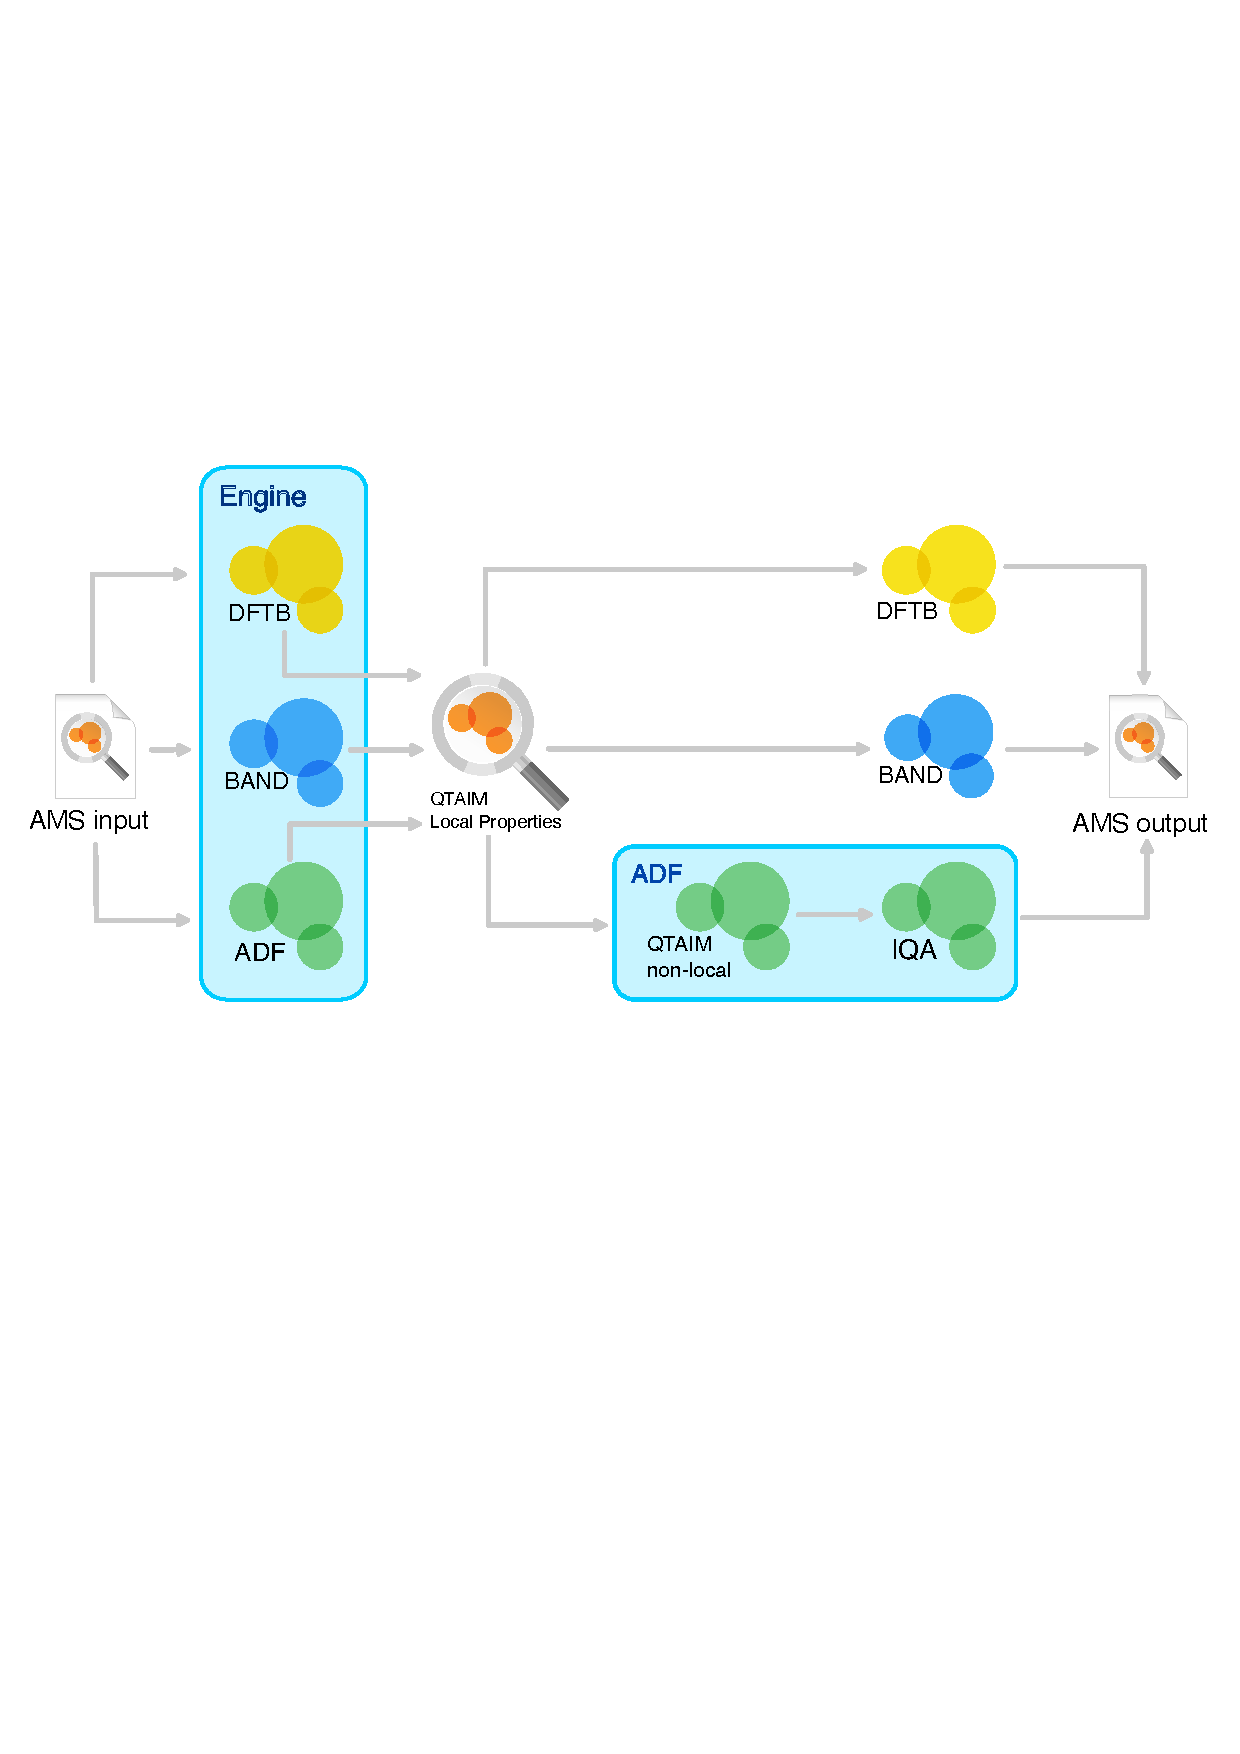
\includegraphics[width=0.75\textwidth]{diagramas/flux.pdf}
  \caption{Workflow from \ams input to output for the engines supporting the
    QTAIM partition.}
  \label{ams_workflow}
\end{figure}

Figure~\ref{ams_modules} provides an overview of the principal \subroutines and
\modules involved in the \gls{QTAIM} implementation. The \ams driver can perform a
single-point calculation with any of the three engines. In the subsequent
post-analysis stage, the \gls{QTAIM} partition is executed. In this workflow, the
\subroutine \texttt{DoSinglePoint} calls \texttt{DoPostSCF}, which first
executes the total energy \subroutine (\texttt{atoten}), followed by the Debye
analysis (\texttt{adebye}). The main \subroutine for producing
\gls{QTAIM} results (\texttt{AIMResults}) requires the outputs of these two
subroutines to compare the dipole moments obtained from the Debye analysis and
from the \gls{QTAIM} partition.

The dipole moment calculation depends on both local properties, computed in
\texttt{ADFAIMCriticalPoints}, and atomic properties, such as the atomic
charges determined by \texttt{UpdateAIMTerms}. Consequently, the
\subroutine responsible for the dipole moment
(\texttt{AIMDipoleMoment}) must be executed only after both
\texttt{ADFAIMCriticalPoints} and \texttt{UpdateAIMTerms} have completed.

\newpage
\vspace*{4cm}
\begin{figure}[h]
  \centering
  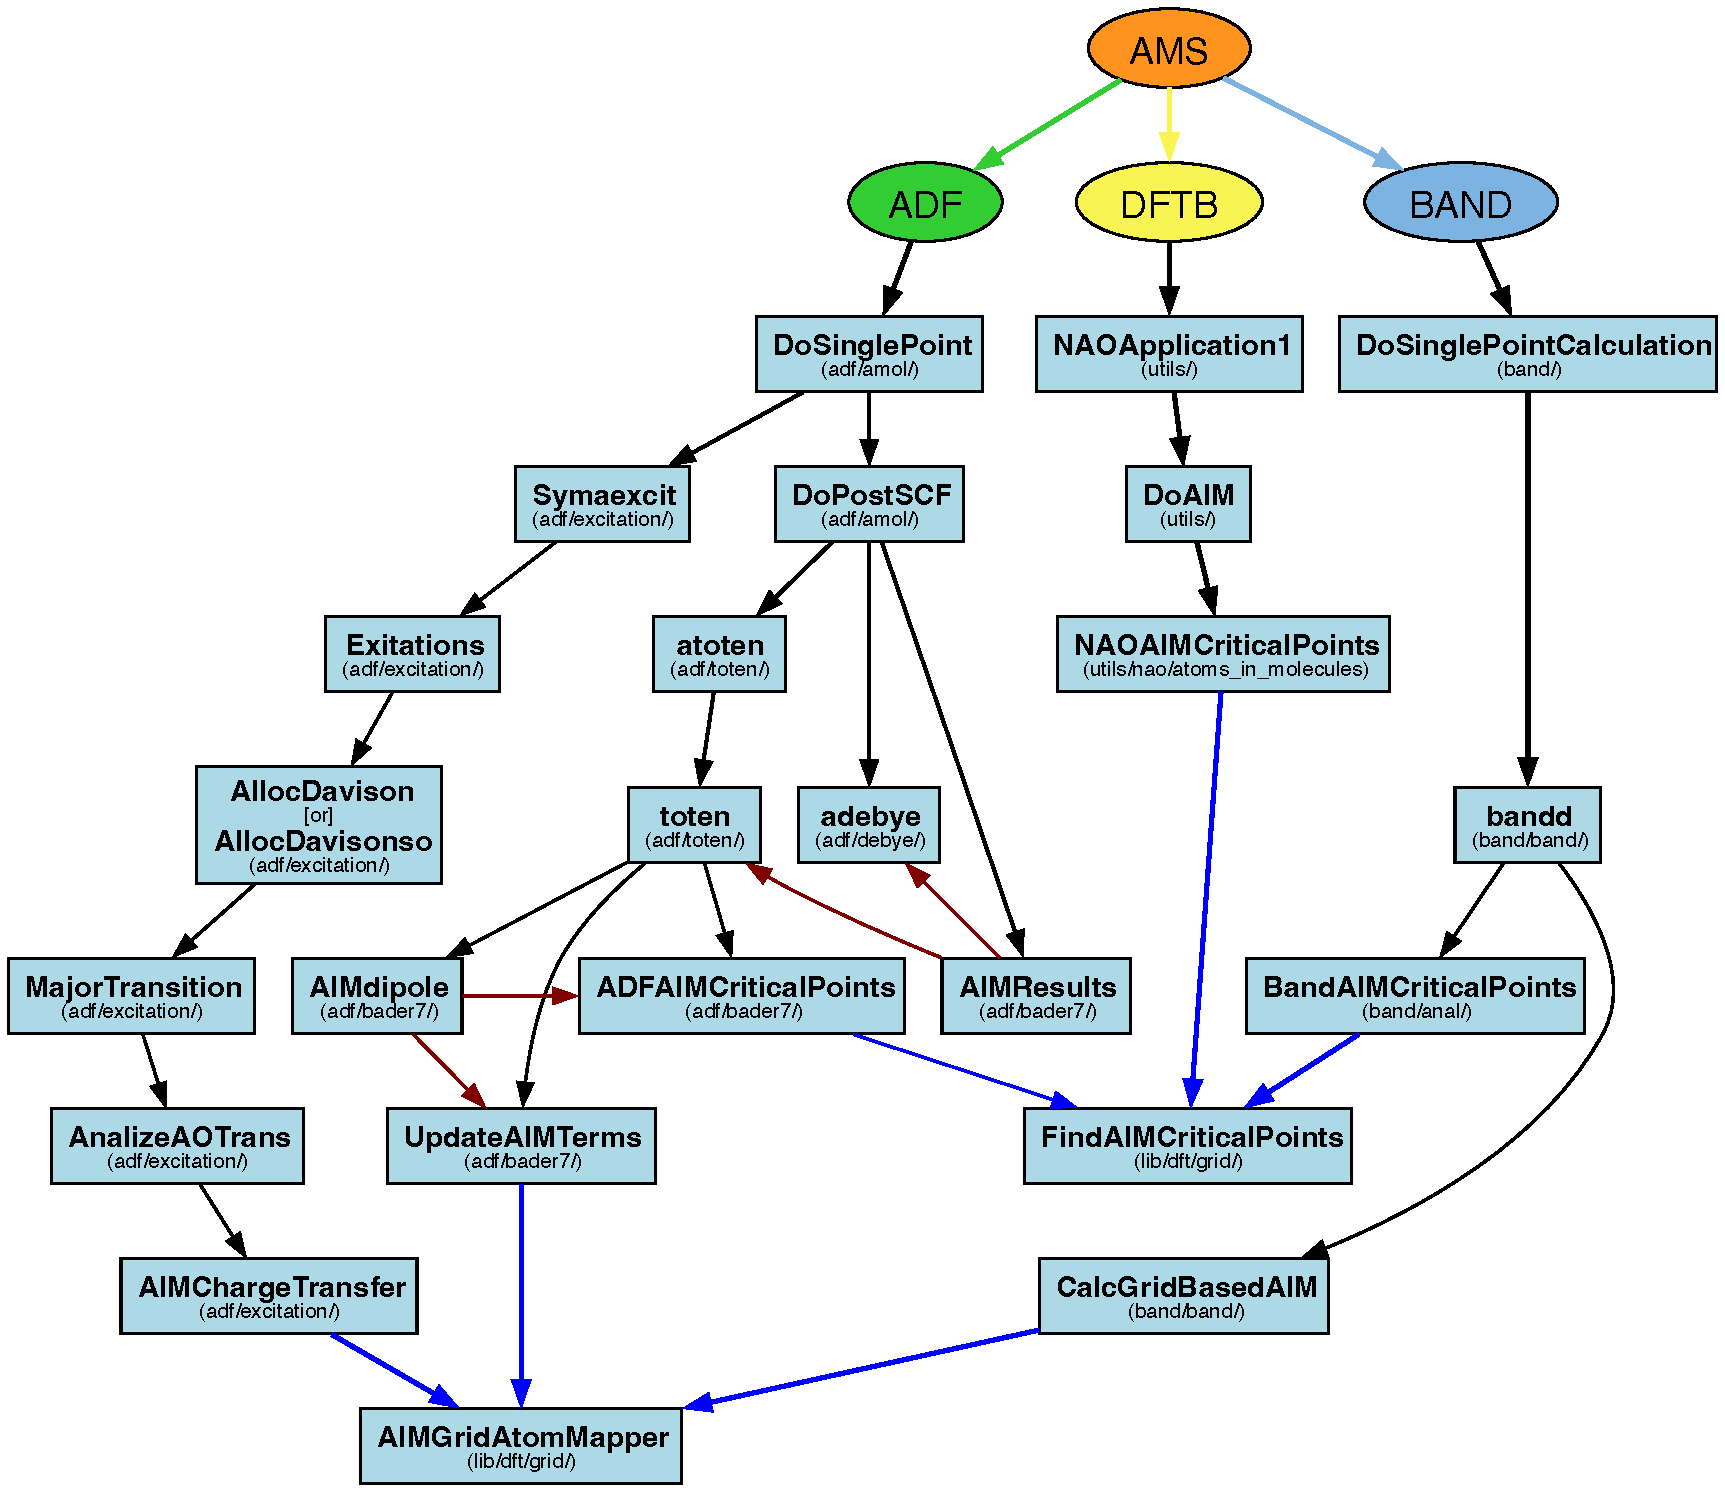
\includegraphics[width=0.9\textwidth]{calls/ams.pdf}
  \caption{The blue arrows indicate the main dependencies; black arrows denote
           subroutine calls; and brown arrows indicate that the main
           subroutine of a module must wait for the execution of the targeted
           subroutines.}
  \label{ams_modules}
\end{figure}

\newpage
\subsection{Descriptors Available in AMS}

The descriptors from the topological analysis (\texttt{AnalysisLevel Normal})
are listed in Table~\ref{aim_descriptors}. For \band, the analysis is more
limited, providing only the electron density and Laplacian for each basin.

\begin{table}[h!]
  \caption{Descriptors available in \adf and \dftb for the Topological Analysis.}
  % -*- coding: utf-8 -*-

\begin{tcolorbox}[tab2,
  tabularx={>{\arraybackslash}m{3.5cm}|>{\arraybackslash}X|>{\arraybackslash}m{1.5cm}},
  title=Descriptors Available in ADF and DFTB for CPs,
  fontupper=\tiny,
  fonttitle=\bfseries,
  boxrule=0.5pt]

  & & \\
  \textbf{Descriptor} & \textbf{Equation} & \textbf{Reference} \\ \hline\hline

  & & \\ [-2mm]
  General Descriptors &
  $\rho, \nabla\rho, \mathbf{H}_\rho, \nabla^2\rho, \diamondsuit \rho, ellepticity $ &
  \\
  & & \\ [-2mm] \hline

  & & \\ [-2mm]
  Metallicity &
  $\xi_m(\mathbf{r}_\mathrm{cp}) = \frac{36(3\pi^2)^{\sfrac{2}{3}}}5\frac{\rho^{\sfrac{5}{3}}}{\nabla^2\rho}$ &
  \cite{Ayers2015} \\
  & & \\ [-2mm] \hline

  %$\wp$

  & & \\ [-2mm]
  Variation Rates & 
  \makecell[l]{
  $\delta u = \frac1{4\pi}\int_\tau\sin\phi\sqrt{\lambda_1^2\sin^2\phi\cos^2\theta + \lambda_2^2\sin^2\phi\sin^2\theta + \lambda_3^2\cos^2\phi}\dd\phi\dd\theta$ \\
  $\delta s = \frac{A_s}{4\pi\rho^{\sfrac{4}{3}}}\int_\tau\sin\phi\sqrt{\lambda_1^2\sin^2\phi\cos^2\theta + \lambda_2^2\sin^2\phi\sin^2\theta + \lambda_3^2\cos^2\phi}\dd\phi\dd\theta$ \\
  $\delta t = \frac{A_t}{4\pi\rho^{\sfrac{7}{6}}}\int_\tau\sin\phi\sqrt{\lambda_1^2\sin^2\phi\cos^2\theta + \lambda_2^2\sin^2\phi\sin^2\theta + \lambda_3^2\cos^2\phi}\dd\phi\dd\theta$
  } &
  \cite{Tognetti2009, Tognetti2014} \\
  & & \\ [-2mm] \hline

  & & \\ [-2mm]
  Inhomogeneites &
  \makecell[l]{
  $l_{s(\mathbf{r}_c)} = \frac1{\langle s' \rangle (\mathbf{r}_c)}$\\
  $l_{e_x(\mathbf{r}_c)} = \sqrt{\sfrac{e_{x(\mathbf{r}_c)}}{\langle \delta e_x \rangle _{\mathbf{r}_c}}}$
  } &
  \cite{Tognetti2013} \\
  & & \\ [-2mm] \hline

  & & \\ [-2mm]
  Abramov's descriptors &
  \makecell[l]{
  $G(\mathbf{r}_\mathrm{cp}) = \sfrac{3}{10}(3\pi^2)^{\sfrac{2}{3}}\rho^{\sfrac{5}{3}} + \sfrac{1}{6}\nabla^2\rho$ \\ 
  $V(\mathbf{r}_\mathrm{cp}) = \sfrac{1}{4}\nabla^2\rho -2G(\mathbf{r}_\mathrm{cp})$ \\
  $H = G(\mathbf{r}_\mathrm{cp}) + V(\mathbf{r}_\mathrm{cp})$
  } & 
  \cite{Abramov1997, Espinosa1998} \\
  & & \\ [-2mm] \hline

  & & \\ [-2mm]
  Uniform Electron Gas &
  \makecell[l]{
  $e^\text{UEG}_x(\mathbf{r}_\mathrm{cp}) = -\frac34\left(\frac3\pi\right)^{\sfrac{1}{3}}\rho^{\sfrac{4}{3}}$ \\
  $e_c^\text{UEG}(\mathbf{r}_\mathrm{cp}) = \frac{a_0 + a_1\rho + a_2\rho^2}{b_0 + b_1\rho + b_2\rho^2}$
  } &
  \cite{Tognetti2014} \\
  & & \\ [-2mm] \hline

  & & \\ [-2mm]
  Variation Rates &
  \makecell[l]{
  $\langle \delta e_x \rangle ^{(2)} = \frac{1}{2\sqrt[3]{(9\pi)}}\rho^{\sfrac{1}{3}}\nabla^2\rho 
  - \frac{\mu\diamondsuit \rho}{16(3\pi^5)^{\sfrac{1}{3}}\rho^{\sfrac{4}{3}}}$\\
  $\langle \delta e_c \rangle ^{(2)} = \frac{a_1b_0 - a_0b_1 + 2(a_2b_0 -a_0b_2)\rho +(a_2b_1 - a_1b_2)\rho^2}{6(b_0 + b_1\rho + b_2\rho^2)^2}
  \times\nabla^2\rho$\\ $\qquad\qquad + \frac{\pi^{\sfrac{1}{3}}\beta_c\diamondsuit \rho}{3^{\sfrac{4}{3}} 16\rho^{\sfrac{4}{3}}}$ \\
  $\langle \delta e_T\rangle^{(2)} = \frac{\pi^{\sfrac{4}{3}}}{4\sqrt[3]{3}}\rho^{\sfrac{2}{3}}\nabla^2\rho + \frac{\diamondsuit \rho}{24\rho}$
  } &
  \cite{Tognetti2014} \\
  & & \\ [-2mm] \hline

  & & \\ [-2mm]
  Locally Compare Ratios &
  \makecell[l]{
  $Q_{xc}(\mathbf{r}_c) = \frac{\langle e_x \rangle ^{(2)}_{\mathbf{r}_c}}{\langle e_c \rangle ^{(2)}_{\mathbf{r}_c}}$\\
  $P_{xc}(\mathbf{r}_c) = \frac{e_x(\mathbf{r}_c)}{e_c(\mathbf{r}_c)}$
  } &
  \cite{Tognetti2014} \\ 
  & &  \\

\end{tcolorbox}


  \label{aim_descriptors}
\end{table}

\newpage
The atomic descriptors (\texttt{AnalysisLevel Extended}) are summarised in
Table~\ref{atomic_descriptors}. Finally, for \texttt{AnalysisLevel Full}, the
localisation and delocalisation indices are computed. An example of the
corresponding output file is provided in Appendix~\ref{output_adf}.

\begin{table}[h!]
  \caption{Descriptors available in \adf and for the Atomic Properties.}
  % -*- coding: utf-8 -*-

\begin{tcolorbox}[tab2,% Integrals
  tabularx={>{\arraybackslash}m{3.5cm}|>{\arraybackslash}X|>{\arraybackslash}m{1.5cm}},
  title=Descriptors Available in ADF for Atomic Basins,
  fontupper=\tiny,
  fonttitle=\bfseries,
  boxrule=0.5pt]

  & & \\
  \textbf{Descriptor} & \textbf{Equation} & \textbf{Reference} \\ \hline\hline

  & & \\ [-2mm]
  Population &
  $\int\rho(\Omega)\dd\tau$ & \cite{bader} \\
  & & \\ [-2mm] \hline

  & & \\ [-2mm]
  Charge &
  $q(\Omega) = Z_\Omega - \int\rho(\Omega)\dd\tau$ & \cite{bader} \\
  & & \\ [-2mm] \hline

  & & \\ [-2mm]
  Spin density &
  $\rho(\uparrow) - \rho(\downarrow)$ & \cite{bader} \\
  & & \\ [-2mm] \hline

  & & \\ [-2mm]
  Laplacian &
  $\int\nabla^2(\rho(\Omega))$ & \cite{bader} \\
  & & \\ [-2mm] \hline

  & & \\ [-2mm]
  Volumen &
  $\int_\text{t}\rho(\Omega)\dd\tau \qquad \text{t} \in \{0.002, 0.001, 0.0004\} \text{a.u.}$ & \cite{bader} \\
  & & \\ [-2mm] \hline

  & & \\ [-2mm]
  Shanon Entropy &
  $H = \int\sigma\ln\sigma\dd\tau$ & \cite{PinedaUrbina2013} \\
  & & \\ [-2mm] \hline

  & & \\ [-2mm]
  Shanon Shape &
  $\frac{H}{\int\rho\dd\tau} + \frac{\ln\int\rho\dd\tau}{\int\rho\dd\tau}\int_\Omega\rho\dd\tau$ & \\
  & & \\ [-2mm] \hline

  & & \\ [-2mm]
  Reyi Shape &
  $-\ln\int_\Omega\rho^2\dd\tau + \ln\int\rho^2\dd\tau$ & \\
  & & \\ [-2mm] \hline

  & & \\ [-2mm]
  Dipole moment &
  $\boldsymbol{\mu}_c = q_\alpha R_\alpha \; ; \; \boldsymbol{\mu}_p = -\int(r-R_\alpha)\rho\dd\tau$ & \cite{Keith} \\
  & & \\ [-2mm] \hline

  & & \\ [-2mm]
  Quadrupole moment &
  $Q_{ij} = \int \rho(\Omega)(3r_ir_j - r^2\delta_{ij})\dd\tau$ & \\
  & & \\ [-2mm] \hline

  & & \\ [-2mm]
  population decomposition over occupied orbitals &
  $\frac{\psi^2_{MO}}{\rho(\Omega)}$ & \\
  & & \\

\end{tcolorbox}


  \label{atomic_descriptors}
\end{table}

\newpage
\subsection{Graphical User Interface (\gls{GUI})}

\begin{wrapfigure}[6]{r}{0.55\textwidth}
\centering
  
\includegraphics[width=0.55\textwidth]{img/gui}
  \label{gui}
\end{wrapfigure}

Although the \gls{QTAIM} partition code had already been implemented in the
\fortran backend, with results written in both human-readable output and binary
files, the \gls{GUI} offered only limited support for visualising the computed
properties. In particular, the display of atomic basin shapes was not
user-friendly.

The main difficulty in rendering atomic basin shapes arises from the
feature that makes the \gls{QTAIM} partition so fast in \ams: the absence of an
explicit calculation of the zero-flux condition (as discussed in previous
sections). The partitioning procedure assigns each grid point to a specific
attractor (or to none), but the basin boundaries cannot be directly extracted
from values computed.

In the previous \gls{GUI} version, atomic basins were visualised by colouring
the corresponding grid points. While functional, this approach often led to
visual clutter, particularly when zooming in or out, as shown in
Figure~\ref{gui_anterior}.

\begin{figure}[h]
  \centering
  \begin{subfigure}{0.48\textwidth}
    \centering
    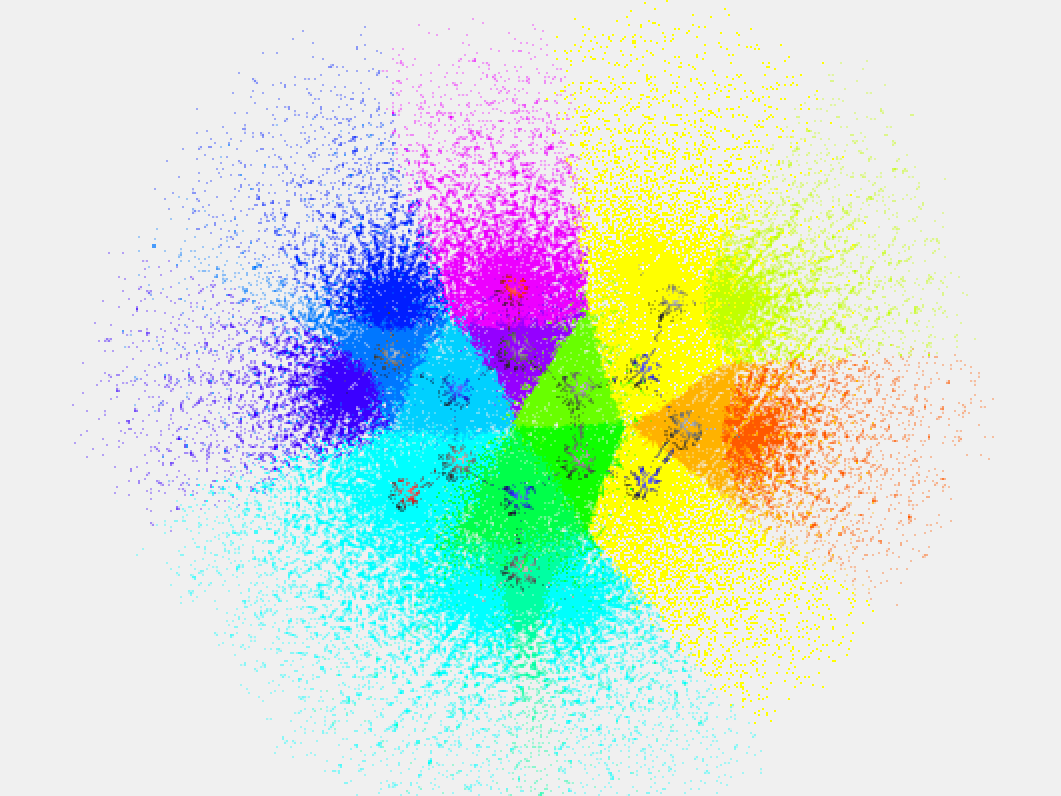
\includegraphics[width=\linewidth]{gui_ss/zoomOut2.png}
    \caption{When zoomed out, the system is obscured by grid points,
      making it difficult to visualise the underlying molecular structure.}
    \label{gui_anterior}
  \end{subfigure}\hfill
  \begin{subfigure}{0.48\textwidth}
    \centering
    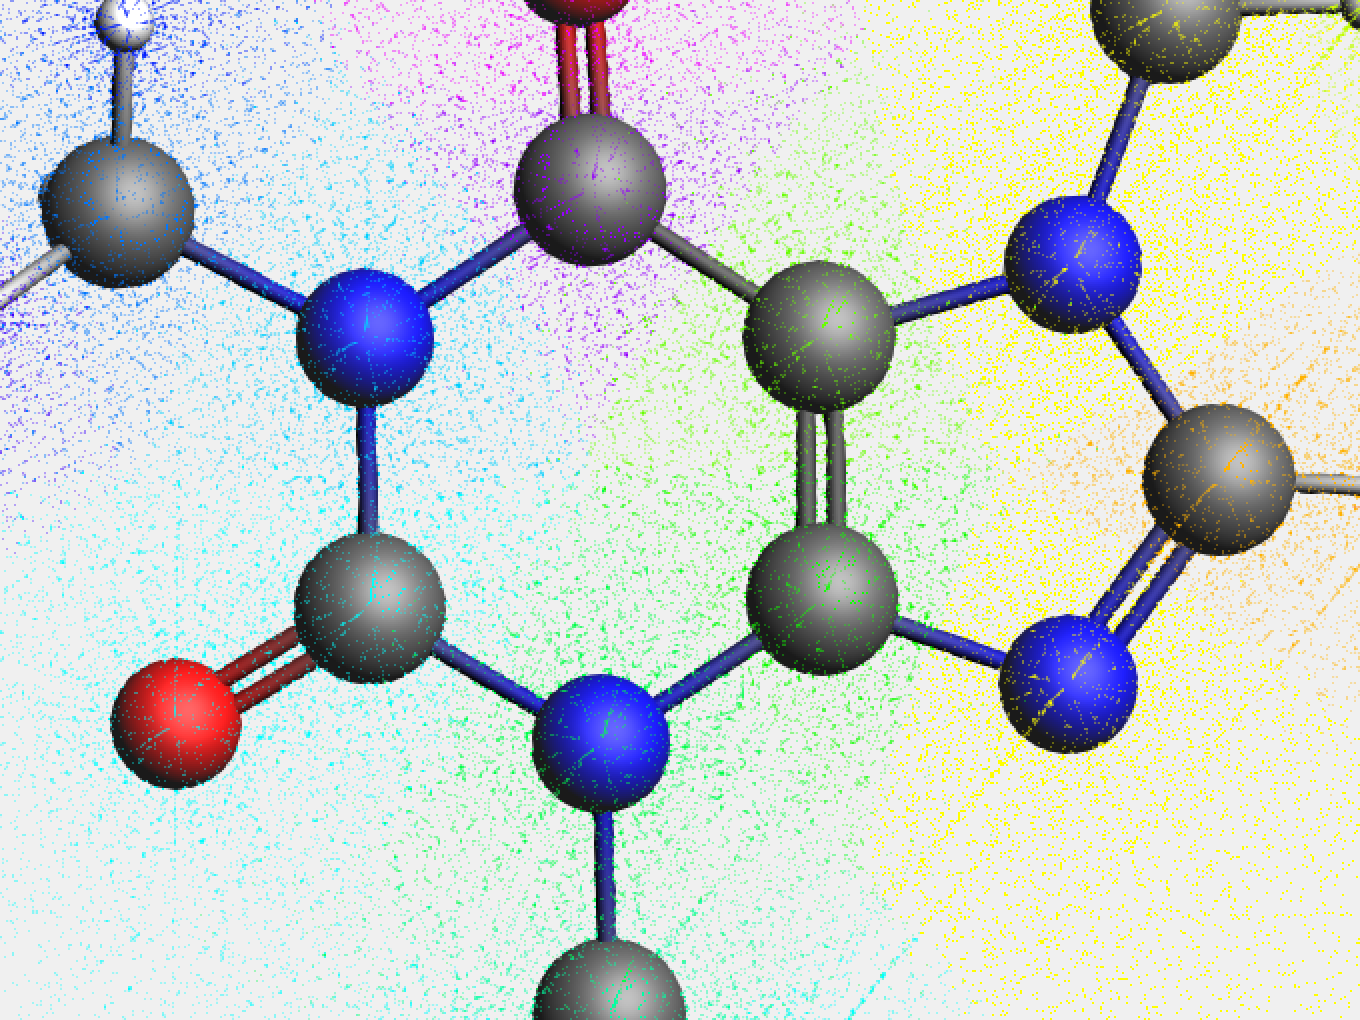
\includegraphics[width=\linewidth]{gui_ss/zoomIn2.png}
    \caption{When zoomed in, the grid points are spaced too far apart,
      and their association becomes difficult for the user.}
    \label{gui_atomic_basin}
  \end{subfigure}
  \caption{Caffeine molecule.}
  \label{water_molecule_gui}
\end{figure}

\newpage
To address this limitation, we implemented a backwards-compatible
\gls{GUI} feature that reconstructs approximate basin surfaces using the
labelled grid points. These shapes are rendered in
\vtk within the \tcl-based \gls{GUI}. A condensed version of the \tcl code is
provided below with comments explaining the main steps of the process.

% -*- coding: utf-8 -*-

\begin{lstlisting}[language=tcl]
    # Read the TAPE10 ...
    # A polygon for every atom
    for {set iatom 0} {$iatom <= $natoms} {incr iatom} {
        # PolyData store the strucuture for every atom
        vtkPolyData $id.t10polydata.$iatom
        lappend VTK($id,ids) $id.t10polydata.$iatom
        $id.t10polydata.$iatom SetPoints $id.t10points
        $id.t10polydata.$iatom SetVerts $id.t10vert.$iatom

        # Sanity check
        if { [$id.t10polydata.$iatom GetNumberOfCells] < 4 } { continue }

        # Solid convex hull of the original points
        vtkDelaunay3D $id.del3d.$iatom
        # Code omitted for brevity ... 

        # Exterior faces; from an unstructured grid to a surface
        vtkDataSetSurfaceFilter $id.surf.$iatom
        # Set the connection for the surface ...

        # More polygons; subdivision
        vtkLoopSubdivisionFilter $id.subdiv.$iatom

        # Set the smoothing parameters ...
        vtkSmoothPolyDataFilter $id.t10smooth1.$iatom

        # Normal vectors [Generated by vtk]
        vtkPolyDataNormals $id.norm.$iatom
        $id.norm.$iatom SetInputConnection [$id.t10smooth.$iatom GetOutputPort]

        # Set the values for opacity and visual appearance
        [$id.t10actor.$iatom GetProperty] SetOpacity 0.4
        # ...
    }
\end{lstlisting}



\newpage
It is worth noting that the implementation could be enhanced by increasing the
number of polygons used to represent the surfaces. However, for large systems
this would incur a significant performance cost. Another possible improvement
is to replace the \vtk-generated normal vectors with those derived from the
gradient of the electron density. While this would not change the resolution,
it would enable more realistic lighting calculations, resulting in smoother
and more visually appealing surfaces. This latter feature has already been
developed but is not yet included in the trunk \branch. It will only be
available for future \ams calculations, as the gradient at each grid point is
not stored in the current binary files.

A comparison of the new and old \gls{GUI} display for atomic basins is shown in
the next Figures~\ref{gui_atomic_basin}.

\begin{figure}[h!]
  \centering
  \begin{subfigure}{0.48\textwidth}
    \centering
    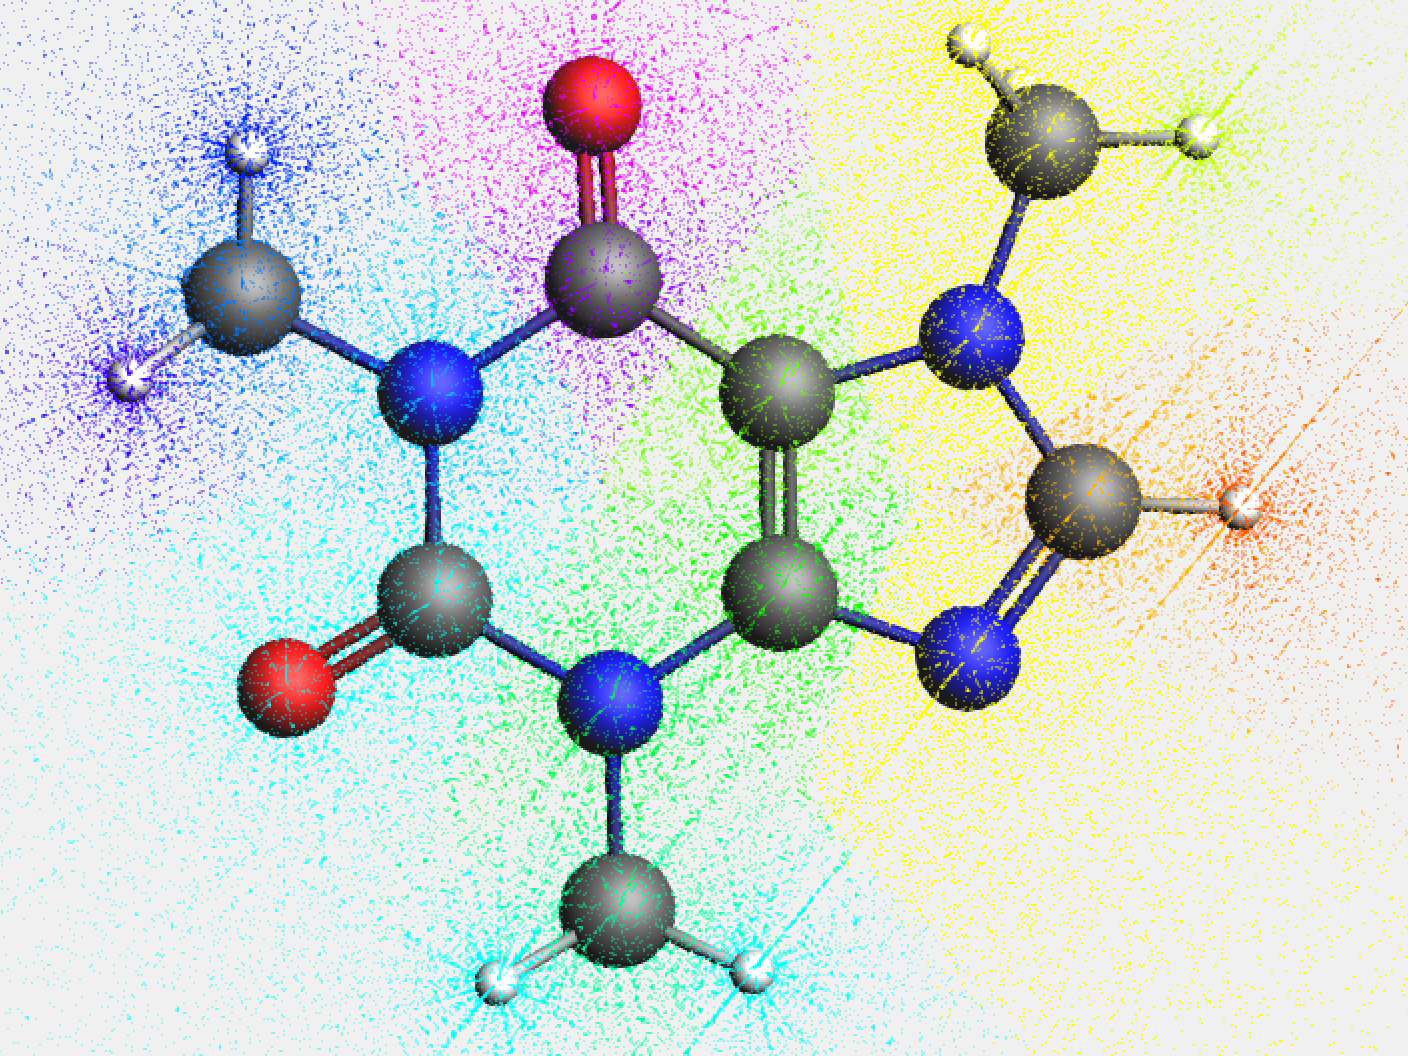
\includegraphics[width=\linewidth]{gui_ss/oldAll2.png}
    \caption{Standard display for all atoms in the previsous \gls{GUI} version.}
  \end{subfigure}
  \begin{subfigure}{0.48\textwidth}
    \centering
    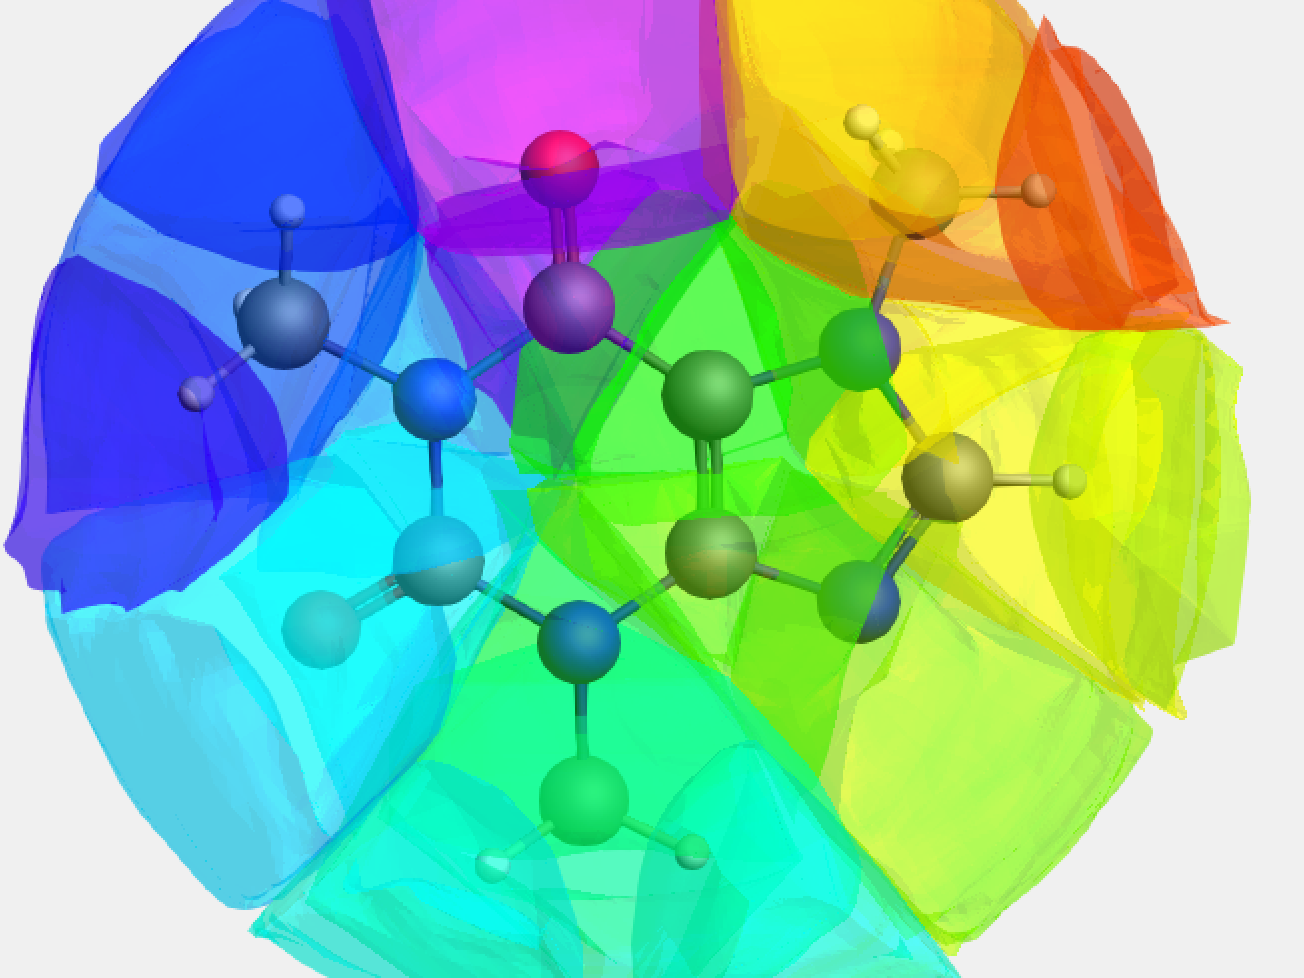
\includegraphics[width=\linewidth]{gui_ss/newAll2.png}
    \caption{Standard display for all atoms in the new \gls{GUI} version.}
  \end{subfigure}

  \begin{subfigure}[t]{0.48\textwidth}
    \centering
    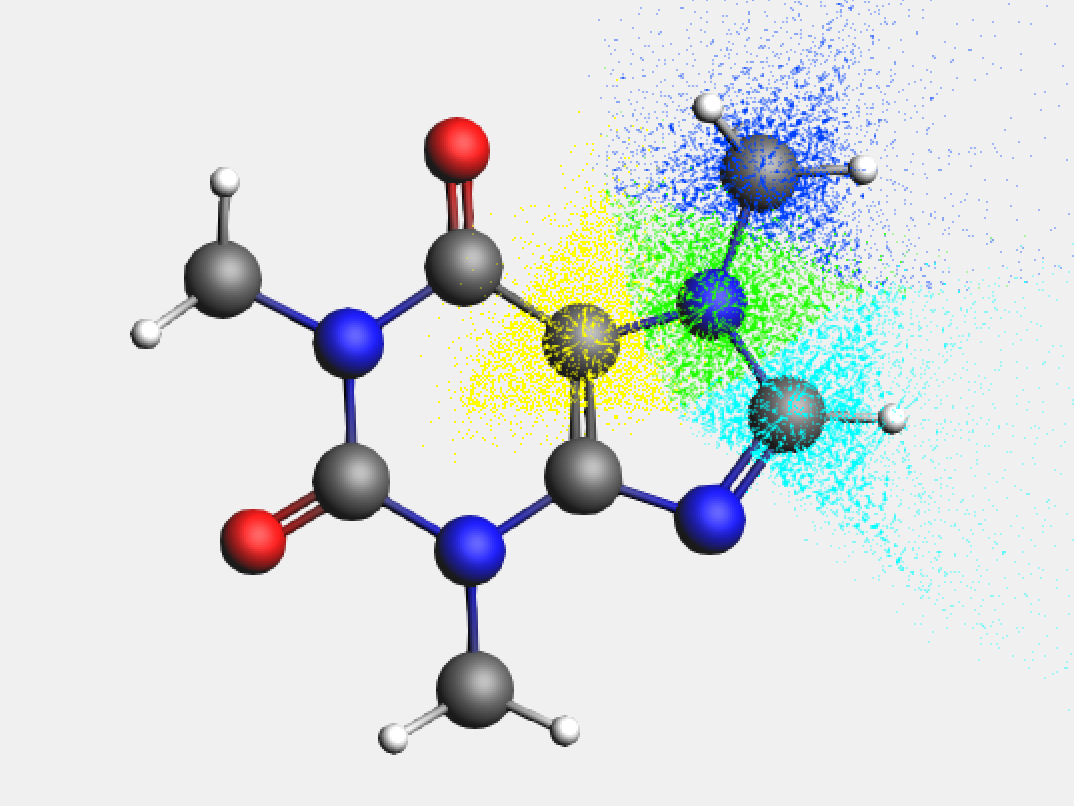
\includegraphics[width=\linewidth]{gui_ss/oldSelected2.png}
    \caption{Only four atoms selected in the previous \gls{GUI} version.}
  \end{subfigure}
  \begin{subfigure}[t]{0.48\textwidth}
    \centering
    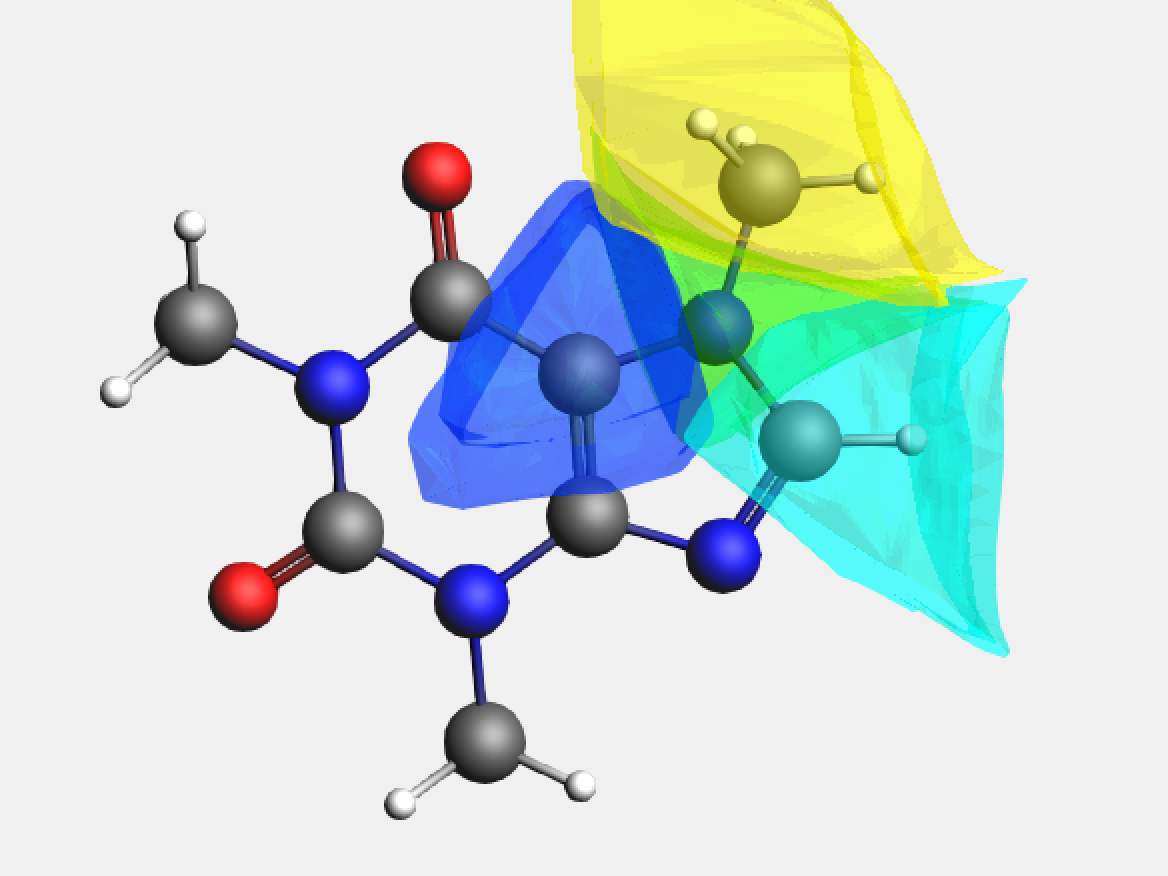
\includegraphics[width=\linewidth]{gui_ss/newSelected2.png}
    \caption{Only four atoms selected in the new \gls{GUI} version.}
  \end{subfigure}
  \caption{Comparison of the new and old \gls{GUI} display for atomic basins, for
    caffeine molecule.}
  \label{gui_atomic_basin}
\end{figure}

